\section{Lektion 30-01-2018}

\begin{enumerate}
	\item Intro
	\item AM Modulation/demodulation
\end{enumerate}

\noindent\fbox{\parbox{\textwidth}{
	\begin{itemize}
	\item \textbf{Pensum:} JV, Ch 1 p 1-6
	\item \textbf{Opgaver:} P.I-1
\end{itemize}
}} \vspace{3mm}

\subsection{Basic Modulation Types and Concepts}

\begin{figure}[!htb]
	\minipage{0.25\textwidth}
	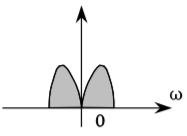
\includegraphics[width=\linewidth]{graphics/1.png}
	\caption*{Original baseband signal}\label{fig:1}
	\endminipage\hfill
	\minipage{0.48\textwidth}
	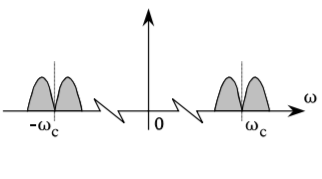
\includegraphics[width=\linewidth]{graphics/2.png}
	\caption*{Transmitted bandpass signal}\label{fig:2}
	\endminipage\hfill
	\minipage{0.25\textwidth}%
	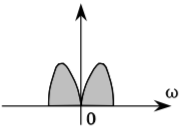
\includegraphics[width=\linewidth]{graphics/3.png}
	\caption*{Reconstructed baseband signal}\label{fig:3}
	\endminipage
\end{figure}

\begin{itemize}
	\item \textbf{Modulation:} Hvordan signaler moduleres ind på bærebølger, der efterfølgende typisk sendes ud som elektromagtetiske signaler via et transmissionsmedie.
	\begin{itemize}
		\item Bandpass signalet er det transmitterede signal til receiveren. 
		\item  Flere baseband signals kan blive transmitteret samtidigt gennem den samme kanal ved forskellige carrier frequencies.
	\end{itemize}
	\item \textbf{Demodulation:} Hvordan det sendte signal demoduleres så det originale signal gendannes. 
	\begin{itemize}
		\item Receiveren gendanner det low-frequency baseband signal.
		\item Scopet af demodulationen afhænger af hvilken type data der bliver sendt.
		\begin{itemize}
			\item \textit{In a radio telephony channel it may suffice at the receiver site to get an output with a power spectrum that contains the dominant part of the input power spectrum.}
			\item  \textit{In a television video channel it is important to reconstruct in time-domain the shape of the signal being send. }
			\item \textit{In digital transmissions, the goal is to rebuild a logical bitstream representation equivalent to the input stream.}
		\end{itemize}
	\end{itemize}
\end{itemize}

\subsection{Amplitude Modulations}
Typer af moduleringer der er egnet for RF communication kaldes
continuous wave modulations, \textbf{CW}.
\begin{itemize}
	\item Baseband information er overlagt en sinusoidal carrier wave med amplitude $A_{c0}$ og vinkelfrekvens $\omega_c$.
	\begin{itemize}
		\item \textit{Carrier} ~\ref{eq:carrier}
		\item \textit{Modulated carrier} ~\ref{eq:modulatedcarrier}
	\end{itemize}
\end{itemize} 

\begin{equation}\label{eq:carrier}
y(t) = A_{c0} \cos(\omega_c t)
\end{equation}

\begin{equation}\label{eq:modulatedcarrier}
y(t) = A(t) \cos(\omega_c t + \phi(t) + \phi_0)
\end{equation}

\begin{itemize}
	\item \textit{The time dependencies of $A(t)$ and $\phi(t)$ in ~\ref{eq:modulatedcarrier} contain the baseband message and the angle $\phi_0$ represents an offset phase for the carrier compared to the timing of the baseband message.} 
	\item \textit{If there is no synchronism between the two, the offset may be set to zero without loss of generality. Eq. ~\ref{eq:modulatedcarrier} is called the envelope-phase representation of a modulated signal.}
\end{itemize}

Den største forskel mellem forskellige modulation typer er hvordan et baseband signal $x(t)$ indeholder det overlagte signal $y(t)$ som er moduleret. Amplitude modulations indebærer \textbf{AM} and \textbf{DSB-SC}.

\subsubsection{AM}
\begin{itemize}
	\item Skalering af signalniveauerne beregnes ved modulation index m.
	\item Med et normaliseret baseband signal $|x(t)|\leq 1$, indebærer betingelsen $m \leq 1$ ( eller $100 \% $ ) et undistorted reproduction af  baseband signalet.
	\begin{itemize}
		\item \textit{m}: modulation index 
	\end{itemize}
	\item Det er let at gendanne baseband signalet fra en AM modulated wave i en receiver med det simple envelope detector circuit. 
\end{itemize} 

\begin{figure} [H]
	\centering
	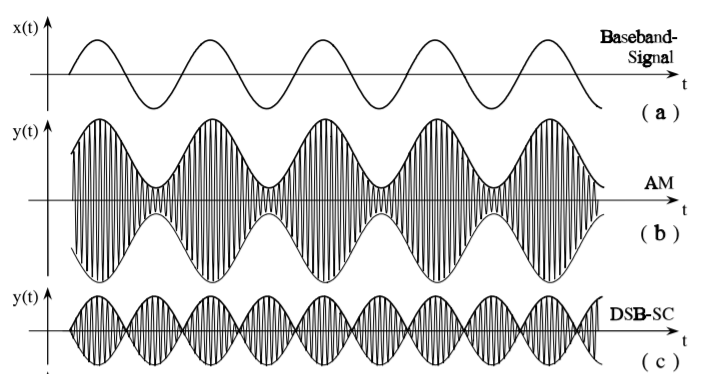
\includegraphics[width=\linewidth]{graphics/4.png}
	\caption{Examples of modulation waveshapes (AM and DSB(-SC)) from a sinusoidal baseband signal $x(t)$.}
	\label{fig:4}
\end{figure}

\begin{itemize}
	\item Amplitude modulation, $\phi(t) = 0$
	\begin{itemize}
		\item \textit{amplitude modulation, AM} ~\ref{eq:AM}
		\item \textit{double-sideband (supressed carrier), DSB/DSB-SC} ~\ref{eq:DSB}
	\end{itemize}
\end{itemize} 

\begin{equation}\label{eq:AM}
y(t) = A_{c0}(1+m x(t)) \cos(\omega_c t)
\end{equation}

\begin{equation}\label{eq:DSB}
y(t) = A_{c0} x(t) \cos(\omega_c t)
\end{equation}

\begin{itemize}
	\item Envelope detectorens low-pass filter bandwidth skal være højere end envelope frekvensen. 
	\item En AM modulated wave har spektrale komponenter fra baseband signalet over og under carrier signalet. 
\end{itemize}

\begin{equation}\label{eq:AM_spectral1}
y(t)_{|AM} = A_{c0}(1+m A_x \cos \omega_x t) \cos \omega_c t \Rrightarrow
\end{equation}

\begin{equation}\label{eq:AM_spectral2}
A_{c0} \cos \omega_c t + \dfrac{A_{c0}}{2}m A_x \cos(\omega_c-\omega_x) t + \dfrac{A_{c0}}{2} m A_x \cos(\omega_c+\omega_x) t
\end{equation}

\begin{figure} [H]
	\centering
	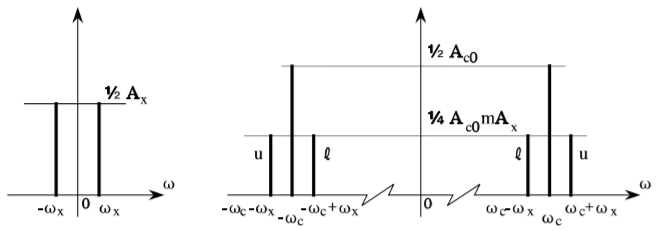
\includegraphics[width=0.85\linewidth]{graphics/5.png}
	\caption{ Spectral components in a double-sided amplitude spectrum of the sinusoidal baseband signal and the AM modulated waveform from Eq. ~\ref{eq:AM_spectral2}. $u$ and $l$ are the	upper and lower sideband components.}
	\label{fig:5}
\end{figure}

\begin{mdframed}[style=exampledefault]
With maximum undistorted modulation, i.e. $m=1$ and $A_x = 1$, the power of the AM modulated wave, say it is a voltage across a \SI{1}{\ohm} resistor, becomes;\\
\begin{equation}\label{eq:AM_ex1}
P_{|AM} = 2 \dfrac{A_{c0}^2}{4} + 4 \dfrac{A_{c0}^2 m^2 A_x^2}{16}
\end{equation}
\begin{center}
	\textit{carrier \qquad envelope}
\end{center}

\begin{equation}\label{eq:ex2}
P_{|AM} = \dfrac{1}{2}A_{c0}^2 + \dfrac{1}{4}A_{c0}^2
\end{equation}
so at most 33\% of the transmitted power contains the message from the baseband signal.
\end{mdframed}

\begin{itemize}
	\item AM modulated signal i frekvens domænet:
	\begin{itemize}
		\item Anvender eulers formel ($\cos 2\pi t \rightarrow e^{j2\pi\omega_c t}+e^{-j2\pi\omega_c t}$)
		\item Fourier transform (gange i tidsdomænet $\cdot$ og folde i frekvenssdomænet $\circledast$) 
	\end{itemize}
\end{itemize}

\begin{figure} [H]
	\centering
	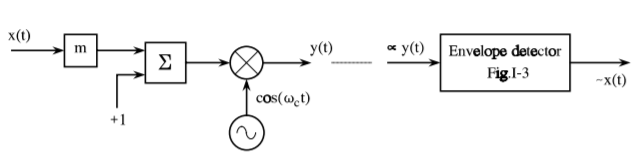
\includegraphics[width=\linewidth]{graphics/6.png}
	\caption{ Block schemes for simple AM modulation (left) and demodulation (right).}
	\label{fig:6}
\end{figure}


\subsubsection{DSB-SC}
DSB moduleringen fra Eq. ~\ref{eq:DSB} har ingen carrier component deraf kommer betegnelsen \textit{suppressed carrier} eller SC.

\begin{equation}\label{eq:DSB_spectral1}
y(t)_{|DSB-SC} = A_{c0} A_x \cos \omega_x t) \cos \omega_c t
\end{equation}

\begin{equation}\label{eq:DSB_spectral2}
y(t)_{|DSB-SC}  = \dfrac{A_{c0}A_x}{2} \cos(\omega_c-\omega_x) t + \dfrac{A_{c0}A_x}{2} \cos(\omega_c+\omega_x) t
\end{equation}

\begin{itemize}
	\item Carrier componenterne indeholder ingen information, derfor er det mere kompliceret at gendanne baseband signalet i receiveren.
	\item For at kunne detektere baseband signalet fra et DSB moduleret
	signal, skal dette signal igen multipliceres med en carrier.
	\begin{itemize}
		\item  Hvis fasen $\phi(t)$ er forskellig fra nul vil
		cosine enten reducerer eller forvrænge signalet.
		\item For at få et predictable result skal oscillatoren i demodulatoren være  synkroniseret med carrier af det modtagede signal. 
		\item \textit{A simple method is to let a fragment of the full carrier - a pilot carrier - follow the signal.}
		\begin{itemize}
			\item Gøres ved at indsætte en konstant $<1$ istedet for $1$.
		\end{itemize}
	\end{itemize}
\end{itemize}

\begin{figure} [H]
	\centering
	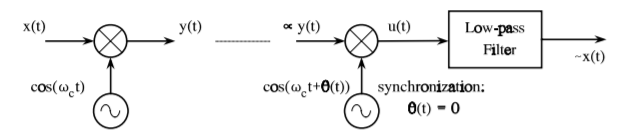
\includegraphics[width=\linewidth]{graphics/7.png}
	\caption{ Block schemes for simple DSB-SC modulation (left) and demodulation (right).}
	\label{fig:7}
\end{figure}
